\begin{frame}
\frametitle{Bundespräsident Gauck zur NSA-Überwachung}
\begin{center}
	\enquote{Wir wissen z.B., dass es nicht so ist, wie bei der Stasi und dem KGB, dass es dicke Aktenbände gibt, wo unsere Gesprächsinhalte alle aufgeschrieben und schön abgeheftet sind. Das ist es nicht.} \par
	Quelle: Gauck, 30.06.2013 im ZDF-Sommerinterview
\end{center}
\end{frame}

\note{Zur Einleitung wird das Zitat vorgelesen. Das Ziel ist, dass die Schüler, im Gegensatz zum Bunderpräsidenten, wissen dass heutzutage alles was an Daten über sie gespeichert wird nicht auf Papier geschieht, sondern abrufbar und verknüpfbar auf Festplatten liegt.}

\begin{frame}
    \frametitle{Stasi vs. NSA}
    \begin{center}
      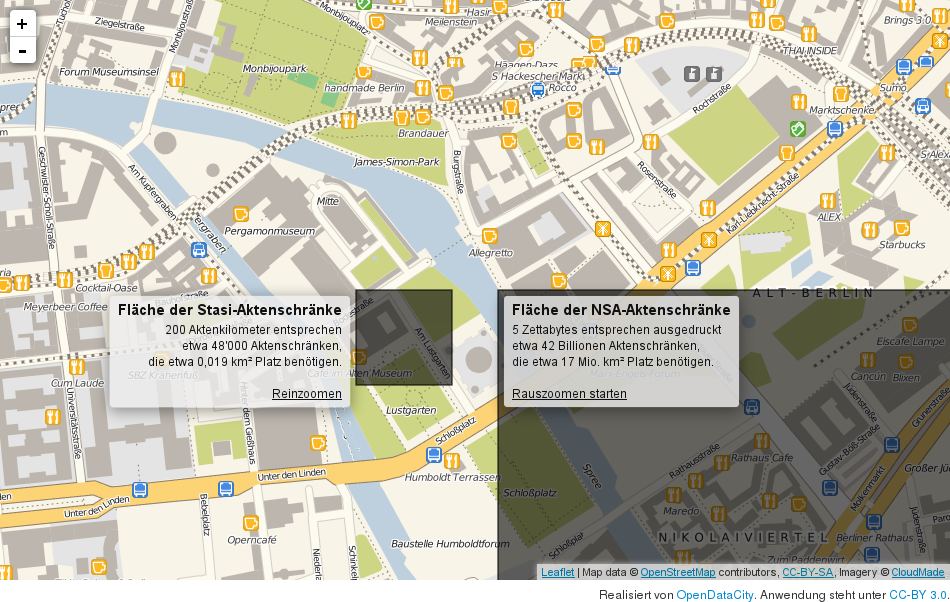
\includegraphics[height=0.7\textheight]{img/akten1.png}
    \end{center}
\end{frame}

\note{Das kleine Quadrat auf der berliner Museumsinsel ist die Fläche, die die Stasiakten einnehmen würden, wenn man sie auf dem Boden auslegen würde. Das größere Quadrat ist nicht komplett sichtbar. Es handelt sich hier um die Fläche, die die Daten der NSA (Stand: vor 3 Jahren) einnehmen würden, wenn man sie ausdrucken und ebenfalls auf dem Boden auslegen würde. Die Schüler sollen raten wie groß das Quadrat ist (übliche Antworten: so groß wie ein Stadtviertel, so groß wie Berlin).}

\begin{frame}
    \frametitle{Stasi vs. NSA}
    \begin{center}
      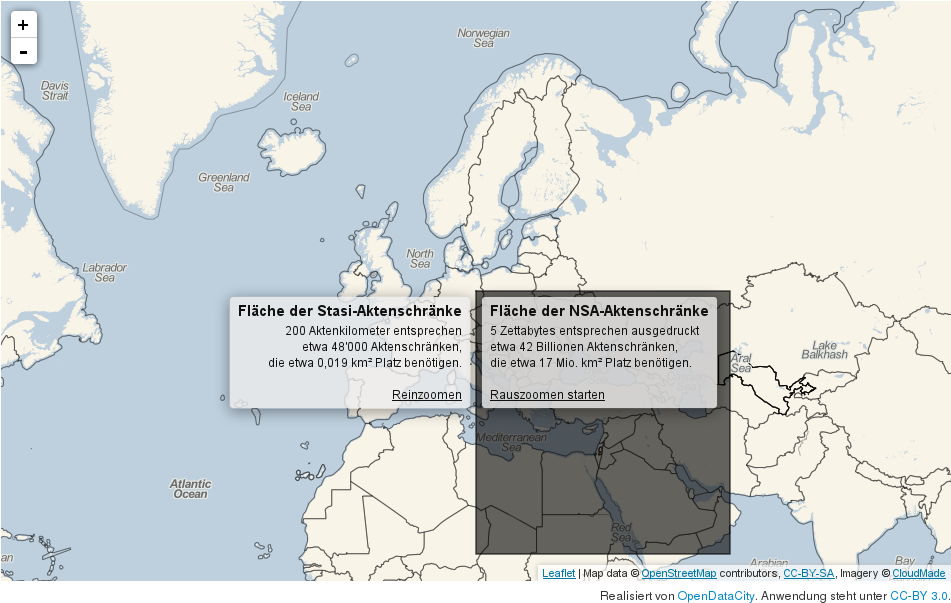
\includegraphics[height=0.7\textheight]{img/akten2.png}
    \end{center}
\end{frame}

\note{Die Auflösung ist meist überraschend, der eingenommene Bereich reicht bis in die Mitte von Afrika hinein und visualisiert sehr deutlich, was technisch heute nicht nur möglich ist sondern auch praktisch geschieht. Eine gute Überleitung ins Thema ist: ``Von jedem Menschen der Erde gibt es Daten in diesem Feld. Wir zeigen euch, wie ihr euren Anteil daran verkleinern könnt''.}
